\documentclass[12pt]{article}
\usepackage[canadien]{babel}
\usepackage[utf8]{inputenc}
\usepackage[T1]{fontenc}
\usepackage{fancyhdr}
\usepackage{graphicx}
\graphicspath{ {./logs/figures/} }
\usepackage{enumerate}
\usepackage{amsmath}
\usepackage{amssymb}
\usepackage{subfigure}
\usepackage{amsmath}
\usepackage{amssymb}
\usepackage[normalem]{ulem}
\useunder{\uline}{\ul}{}
\usepackage{float}
\usepackage{bm}
\usepackage{url}
\usepackage[dvipsnames]{xcolor}
\usepackage{todonotes}
\usepackage{hyperref}
\usepackage{monpackage}

% If your paper is accepted, change the options for the package
% aistats2e as follows:
%
%\usepackage[accepted]{aistats2e}
%
% This option will print headings for the title of your paper and
% headings for the authors names, plus a copyright note at the end of
% the first column of the first page.
\setlength{\parindent}{0cm}
\addtolength{\oddsidemargin}{-2cm}
\addtolength{\evensidemargin}{-2cm}
\setlength{\textwidth}{17.78cm}
\addtolength{\topmargin}{-2.25cm}
\setlength{\textheight}{23.24cm}
\addtolength{\parskip}{5mm}
\pagestyle{fancy}

%************
%* COMMANDS *
%************

%%%%% NEW MATH DEFINITIONS %%%%%

% Mark sections of captions for referring to divisions of figures
\newcommand{\figleft}{{\em (Left)}}
\newcommand{\figcenter}{{\em (Center)}}
\newcommand{\figright}{{\em (Right)}}
\newcommand{\figtop}{{\em (Top)}}
\newcommand{\figbottom}{{\em (Bottom)}}
\newcommand{\captiona}{{\em (a)}}
\newcommand{\captionb}{{\em (b)}}
\newcommand{\captionc}{{\em (c)}}
\newcommand{\captiond}{{\em (d)}}

% Highlight a newly defined term
\newcommand{\newterm}[1]{{\bf #1}}


% Figure reference, lower-case.
\def\figref#1{figure~\ref{#1}}
% Figure reference, capital. For start of sentence
\def\Figref#1{Figure~\ref{#1}}
\def\twofigref#1#2{figures \ref{#1} and \ref{#2}}
\def\quadfigref#1#2#3#4{figures \ref{#1}, \ref{#2}, \ref{#3} and \ref{#4}}
% Section reference, lower-case.
\def\secref#1{section~\ref{#1}}
% Section reference, capital.
\def\Secref#1{Section~\ref{#1}}
% Reference to two sections.
\def\twosecrefs#1#2{sections \ref{#1} and \ref{#2}}
% Reference to three sections.
\def\secrefs#1#2#3{sections \ref{#1}, \ref{#2} and \ref{#3}}
% Reference to an equation, lower-case.
\def\eqref#1{equation~\ref{#1}}
% Reference to an equation, upper case
\def\Eqref#1{Equation~\ref{#1}}
% A raw reference to an equation---avoid using if possible
\def\plaineqref#1{\ref{#1}}
% Reference to a chapter, lower-case.
\def\chapref#1{chapter~\ref{#1}}
% Reference to an equation, upper case.
\def\Chapref#1{Chapter~\ref{#1}}
% Reference to a range of chapters
\def\rangechapref#1#2{chapters\ref{#1}--\ref{#2}}
% Reference to an algorithm, lower-case.
\def\algref#1{algorithm~\ref{#1}}
% Reference to an algorithm, upper case.
\def\Algref#1{Algorithm~\ref{#1}}
\def\twoalgref#1#2{algorithms \ref{#1} and \ref{#2}}
\def\Twoalgref#1#2{Algorithms \ref{#1} and \ref{#2}}
% Reference to a part, lower case
\def\partref#1{part~\ref{#1}}
% Reference to a part, upper case
\def\Partref#1{Part~\ref{#1}}
\def\twopartref#1#2{parts \ref{#1} and \ref{#2}}

\def\ceil#1{\lceil #1 \rceil}
\def\floor#1{\lfloor #1 \rfloor}
\def\1{\bm{1}}
\newcommand{\train}{\mathcal{D}}
\newcommand{\valid}{\mathcal{D_{\mathrm{valid}}}}
\newcommand{\test}{\mathcal{D_{\mathrm{test}}}}

\def\eps{{\epsilon}}


% Random variables
\def\reta{{\textnormal{$\eta$}}}
\def\ra{{\textnormal{a}}}
\def\rb{{\textnormal{b}}}
\def\rc{{\textnormal{c}}}
\def\rd{{\textnormal{d}}}
\def\re{{\textnormal{e}}}
\def\rf{{\textnormal{f}}}
\def\rg{{\textnormal{g}}}
\def\rh{{\textnormal{h}}}
\def\ri{{\textnormal{i}}}
\def\rj{{\textnormal{j}}}
\def\rk{{\textnormal{k}}}
\def\rl{{\textnormal{l}}}
% rm is already a command, just don't name any random variables m
\def\rn{{\textnormal{n}}}
\def\ro{{\textnormal{o}}}
\def\rp{{\textnormal{p}}}
\def\rq{{\textnormal{q}}}
\def\rr{{\textnormal{r}}}
\def\rs{{\textnormal{s}}}
\def\rt{{\textnormal{t}}}
\def\ru{{\textnormal{u}}}
\def\rv{{\textnormal{v}}}
\def\rw{{\textnormal{w}}}
\def\rx{{\textnormal{x}}}
\def\ry{{\textnormal{y}}}
\def\rz{{\textnormal{z}}}

% Random vectors
\def\rvepsilon{{\mathbf{\epsilon}}}
\def\rvtheta{{\mathbf{\theta}}}
\def\rva{{\mathbf{a}}}
\def\rvb{{\mathbf{b}}}
\def\rvc{{\mathbf{c}}}
\def\rvd{{\mathbf{d}}}
\def\rve{{\mathbf{e}}}
\def\rvf{{\mathbf{f}}}
\def\rvg{{\mathbf{g}}}
\def\rvh{{\mathbf{h}}}
\def\rvu{{\mathbf{i}}}
\def\rvj{{\mathbf{j}}}
\def\rvk{{\mathbf{k}}}
\def\rvl{{\mathbf{l}}}
\def\rvm{{\mathbf{m}}}
\def\rvn{{\mathbf{n}}}
\def\rvo{{\mathbf{o}}}
\def\rvp{{\mathbf{p}}}
\def\rvq{{\mathbf{q}}}
\def\rvr{{\mathbf{r}}}
\def\rvs{{\mathbf{s}}}
\def\rvt{{\mathbf{t}}}
\def\rvu{{\mathbf{u}}}
\def\rvv{{\mathbf{v}}}
\def\rvw{{\mathbf{w}}}
\def\rvx{{\mathbf{x}}}
\def\rvy{{\mathbf{y}}}
\def\rvz{{\mathbf{z}}}

% Elements of random vectors
\def\erva{{\textnormal{a}}}
\def\ervb{{\textnormal{b}}}
\def\ervc{{\textnormal{c}}}
\def\ervd{{\textnormal{d}}}
\def\erve{{\textnormal{e}}}
\def\ervf{{\textnormal{f}}}
\def\ervg{{\textnormal{g}}}
\def\ervh{{\textnormal{h}}}
\def\ervi{{\textnormal{i}}}
\def\ervj{{\textnormal{j}}}
\def\ervk{{\textnormal{k}}}
\def\ervl{{\textnormal{l}}}
\def\ervm{{\textnormal{m}}}
\def\ervn{{\textnormal{n}}}
\def\ervo{{\textnormal{o}}}
\def\ervp{{\textnormal{p}}}
\def\ervq{{\textnormal{q}}}
\def\ervr{{\textnormal{r}}}
\def\ervs{{\textnormal{s}}}
\def\ervt{{\textnormal{t}}}
\def\ervu{{\textnormal{u}}}
\def\ervv{{\textnormal{v}}}
\def\ervw{{\textnormal{w}}}
\def\ervx{{\textnormal{x}}}
\def\ervy{{\textnormal{y}}}
\def\ervz{{\textnormal{z}}}

% Random matrices
\def\rmA{{\mathbf{A}}}
\def\rmB{{\mathbf{B}}}
\def\rmC{{\mathbf{C}}}
\def\rmD{{\mathbf{D}}}
\def\rmE{{\mathbf{E}}}
\def\rmF{{\mathbf{F}}}
\def\rmG{{\mathbf{G}}}
\def\rmH{{\mathbf{H}}}
\def\rmI{{\mathbf{I}}}
\def\rmJ{{\mathbf{J}}}
\def\rmK{{\mathbf{K}}}
\def\rmL{{\mathbf{L}}}
\def\rmM{{\mathbf{M}}}
\def\rmN{{\mathbf{N}}}
\def\rmO{{\mathbf{O}}}
\def\rmP{{\mathbf{P}}}
\def\rmQ{{\mathbf{Q}}}
\def\rmR{{\mathbf{R}}}
\def\rmS{{\mathbf{S}}}
\def\rmT{{\mathbf{T}}}
\def\rmU{{\mathbf{U}}}
\def\rmV{{\mathbf{V}}}
\def\rmW{{\mathbf{W}}}
\def\rmX{{\mathbf{X}}}
\def\rmY{{\mathbf{Y}}}
\def\rmZ{{\mathbf{Z}}}

% Elements of random matrices
\def\ermA{{\textnormal{A}}}
\def\ermB{{\textnormal{B}}}
\def\ermC{{\textnormal{C}}}
\def\ermD{{\textnormal{D}}}
\def\ermE{{\textnormal{E}}}
\def\ermF{{\textnormal{F}}}
\def\ermG{{\textnormal{G}}}
\def\ermH{{\textnormal{H}}}
\def\ermI{{\textnormal{I}}}
\def\ermJ{{\textnormal{J}}}
\def\ermK{{\textnormal{K}}}
\def\ermL{{\textnormal{L}}}
\def\ermM{{\textnormal{M}}}
\def\ermN{{\textnormal{N}}}
\def\ermO{{\textnormal{O}}}
\def\ermP{{\textnormal{P}}}
\def\ermQ{{\textnormal{Q}}}
\def\ermR{{\textnormal{R}}}
\def\ermS{{\textnormal{S}}}
\def\ermT{{\textnormal{T}}}
\def\ermU{{\textnormal{U}}}
\def\ermV{{\textnormal{V}}}
\def\ermW{{\textnormal{W}}}
\def\ermX{{\textnormal{X}}}
\def\ermY{{\textnormal{Y}}}
\def\ermZ{{\textnormal{Z}}}

% Vectors
\def\vzero{{\bm{0}}}
\def\vone{{\bm{1}}}
\def\vmu{{\bm{\mu}}}
\def\vtheta{{\bm{\theta}}}
\def\va{{\bm{a}}}
\def\vb{{\bm{b}}}
\def\vc{{\bm{c}}}
\def\vd{{\bm{d}}}
\def\ve{{\bm{e}}}
\def\vf{{\bm{f}}}
\def\vg{{\bm{g}}}
\def\vh{{\bm{h}}}
\def\vi{{\bm{i}}}
\def\vj{{\bm{j}}}
\def\vk{{\bm{k}}}
\def\vl{{\bm{l}}}
\def\vm{{\bm{m}}}
\def\vn{{\bm{n}}}
\def\vo{{\bm{o}}}
\def\vp{{\bm{p}}}
\def\vq{{\bm{q}}}
\def\vr{{\bm{r}}}
\def\vs{{\bm{s}}}
\def\vt{{\bm{t}}}
\def\vu{{\bm{u}}}
\def\vv{{\bm{v}}}
\def\vw{{\bm{w}}}
\def\vx{{\bm{x}}}
\def\vy{{\bm{y}}}
\def\vz{{\bm{z}}}

% Elements of vectors
\def\evalpha{{\alpha}}
\def\evbeta{{\beta}}
\def\evepsilon{{\epsilon}}
\def\evlambda{{\lambda}}
\def\evomega{{\omega}}
\def\evmu{{\mu}}
\def\evpsi{{\psi}}
\def\evsigma{{\sigma}}
\def\evtheta{{\theta}}
\def\eva{{a}}
\def\evb{{b}}
\def\evc{{c}}
\def\evd{{d}}
\def\eve{{e}}
\def\evf{{f}}
\def\evg{{g}}
\def\evh{{h}}
\def\evi{{i}}
\def\evj{{j}}
\def\evk{{k}}
\def\evl{{l}}
\def\evm{{m}}
\def\evn{{n}}
\def\evo{{o}}
\def\evp{{p}}
\def\evq{{q}}
\def\evr{{r}}
\def\evs{{s}}
\def\evt{{t}}
\def\evu{{u}}
\def\evv{{v}}
\def\evw{{w}}
\def\evx{{x}}
\def\evy{{y}}
\def\evz{{z}}

% Matrix
\def\mA{{\bm{A}}}
\def\mB{{\bm{B}}}
\def\mC{{\bm{C}}}
\def\mD{{\bm{D}}}
\def\mE{{\bm{E}}}
\def\mF{{\bm{F}}}
\def\mG{{\bm{G}}}
\def\mH{{\bm{\text{\textbf{H}}}}}
\def\mI{{\bm{I}}}
\def\mJ{{\bm{J}}}
\def\mK{{\bm{K}}}
\def\mL{{\bm{L}}}
\def\mM{{\bm{M}}}
\def\mN{{\bm{N}}}
\def\mO{{\bm{O}}}
\def\mP{{\bm{P}}}
\def\mQ{{\bm{Q}}}
\def\mR{{\bm{R}}}
\def\mS{{\bm{S}}}
\def\mT{{\bm{T}}}
\def\mU{{\bm{U}}}
\def\mV{{\bm{V}}}
\def\mW{{\bm{W}}}
\def\mX{{\bm{X}}}
\def\mY{{\bm{Y}}}
\def\mZ{{\bm{Z}}}
\def\mBeta{{\bm{\beta}}}
\def\mPhi{{\bm{\Phi}}}
\def\mLambda{{\bm{\Lambda}}}
\def\mSigma{{\bm{\Sigma}}}

% Tensor
\DeclareMathAlphabet{\mathsfit}{\encodingdefault}{\sfdefault}{m}{sl}
\SetMathAlphabet{\mathsfit}{bold}{\encodingdefault}{\sfdefault}{bx}{n}
\newcommand{\tens}[1]{\bm{\mathsfit{#1}}}
\def\tA{{\tens{A}}}
\def\tB{{\tens{B}}}
\def\tC{{\tens{C}}}
\def\tD{{\tens{D}}}
\def\tE{{\tens{E}}}
\def\tF{{\tens{F}}}
\def\tG{{\tens{G}}}
\def\tH{{\tens{H}}}
\def\tI{{\tens{I}}}
\def\tJ{{\tens{J}}}
\def\tK{{\tens{K}}}
\def\tL{{\tens{L}}}
\def\tM{{\tens{M}}}
\def\tN{{\tens{N}}}
\def\tO{{\tens{O}}}
\def\tP{{\tens{P}}}
\def\tQ{{\tens{Q}}}
\def\tR{{\tens{R}}}
\def\tS{{\tens{S}}}
\def\tT{{\tens{T}}}
\def\tU{{\tens{U}}}
\def\tV{{\tens{V}}}
\def\tW{{\tens{W}}}
\def\tX{{\tens{X}}}
\def\tY{{\tens{Y}}}
\def\tZ{{\tens{Z}}}


% Graph
\def\gA{{\mathcal{A}}}
\def\gB{{\mathcal{B}}}
\def\gC{{\mathcal{C}}}
\def\gD{{\mathcal{D}}}
\def\gE{{\mathcal{E}}}
\def\gF{{\mathcal{F}}}
\def\gG{{\mathcal{G}}}
\def\gH{{\mathcal{H}}}
\def\gI{{\mathcal{I}}}
\def\gJ{{\mathcal{J}}}
\def\gK{{\mathcal{K}}}
\def\gL{{\mathcal{L}}}
\def\gM{{\mathcal{M}}}
\def\gN{{\mathcal{N}}}
\def\gO{{\mathcal{O}}}
\def\gP{{\mathcal{P}}}
\def\gQ{{\mathcal{Q}}}
\def\gR{{\mathcal{R}}}
\def\gS{{\mathcal{S}}}
\def\gT{{\mathcal{T}}}
\def\gU{{\mathcal{U}}}
\def\gV{{\mathcal{V}}}
\def\gW{{\mathcal{W}}}
\def\gX{{\mathcal{X}}}
\def\gY{{\mathcal{Y}}}
\def\gZ{{\mathcal{Z}}}

% Sets
\def\sA{{\mathbb{A}}}
\def\sB{{\mathbb{B}}}
\def\sC{{\mathbb{C}}}
\def\sD{{\mathbb{D}}}
% Don't use a set called E, because this would be the same as our symbol
% for expectation.
\def\sF{{\mathbb{F}}}
\def\sG{{\mathbb{G}}}
\def\sH{{\mathbb{H}}}
\def\sI{{\mathbb{I}}}
\def\sJ{{\mathbb{J}}}
\def\sK{{\mathbb{K}}}
\def\sL{{\mathbb{L}}}
\def\sM{{\mathbb{M}}}
\def\sN{{\mathbb{N}}}
\def\sO{{\mathbb{O}}}
\def\sP{{\mathbb{P}}}
\def\sQ{{\mathbb{Q}}}
\def\sR{{\mathbb{R}}}
\def\sS{{\mathbb{S}}}
\def\sT{{\mathbb{T}}}
\def\sU{{\mathbb{U}}}
\def\sV{{\mathbb{V}}}
\def\sW{{\mathbb{W}}}
\def\sX{{\mathbb{X}}}
\def\sY{{\mathbb{Y}}}
\def\sZ{{\mathbb{Z}}}

% Entries of a matrix
\def\emLambda{{\Lambda}}
\def\emA{{A}}
\def\emB{{B}}
\def\emC{{C}}
\def\emD{{D}}
\def\emE{{E}}
\def\emF{{F}}
\def\emG{{G}}
\def\emH{{H}}
\def\emI{{I}}
\def\emJ{{J}}
\def\emK{{K}}
\def\emL{{L}}
\def\emM{{M}}
\def\emN{{N}}
\def\emO{{O}}
\def\emP{{P}}
\def\emQ{{Q}}
\def\emR{{R}}
\def\emS{{S}}
\def\emT{{T}}
\def\emU{{U}}
\def\emV{{V}}
\def\emW{{W}}
\def\emX{{X}}
\def\emY{{Y}}
\def\emZ{{Z}}
\def\emSigma{{\Sigma}}

% entries of a tensor
% Same font as tensor, without \bm wrapper
\newcommand{\etens}[1]{\mathsfit{#1}}
\def\etLambda{{\etens{\Lambda}}}
\def\etA{{\etens{A}}}
\def\etB{{\etens{B}}}
\def\etC{{\etens{C}}}
\def\etD{{\etens{D}}}
\def\etE{{\etens{E}}}
\def\etF{{\etens{F}}}
\def\etG{{\etens{G}}}
\def\etH{{\etens{H}}}
\def\etI{{\etens{I}}}
\def\etJ{{\etens{J}}}
\def\etK{{\etens{K}}}
\def\etL{{\etens{L}}}
\def\etM{{\etens{M}}}
\def\etN{{\etens{N}}}
\def\etO{{\etens{O}}}
\def\etP{{\etens{P}}}
\def\etQ{{\etens{Q}}}
\def\etR{{\etens{R}}}
\def\etS{{\etens{S}}}
\def\etT{{\etens{T}}}
\def\etU{{\etens{U}}}
\def\etV{{\etens{V}}}
\def\etW{{\etens{W}}}
\def\etX{{\etens{X}}}
\def\etY{{\etens{Y}}}
\def\etZ{{\etens{Z}}}

% The true underlying data generating distribution
\newcommand{\pdata}{p_{\rm{data}}}
% The empirical distribution defined by the training set
\newcommand{\ptrain}{\hat{p}_{\rm{data}}}
\newcommand{\Ptrain}{\hat{P}_{\rm{data}}}
% The model distribution
\newcommand{\pmodel}{p_{\rm{model}}}
\newcommand{\Pmodel}{P_{\rm{model}}}
\newcommand{\ptildemodel}{\tilde{p}_{\rm{model}}}
% Stochastic autoencoder distributions
\newcommand{\pencode}{p_{\rm{encoder}}}
\newcommand{\pdecode}{p_{\rm{decoder}}}
\newcommand{\precons}{p_{\rm{reconstruct}}}

\newcommand{\laplace}{\mathrm{Laplace}} % Laplace distribution

\newcommand{\E}{\mathbb{E}}
\newcommand{\Ls}{\mathcal{L}}
\newcommand{\R}{\mathbb{R}}
\newcommand{\emp}{\tilde{p}}
\newcommand{\lr}{\alpha}
\newcommand{\reg}{\lambda}
\newcommand{\rect}{\mathrm{rectifier}}
\newcommand{\softmax}{\mathrm{softmax}}
\newcommand{\sigmoid}{\sigma}
\newcommand{\softplus}{\zeta}
\newcommand{\KL}{D_{\mathrm{KL}}}
\newcommand{\Var}{\mathrm{Var}}
\newcommand{\standarderror}{\mathrm{SE}}
\newcommand{\Cov}{\mathrm{Cov}}
% Wolfram Mathworld says $L^2$ is for function spaces and $\ell^2$ is for vectors
% But then they seem to use $L^2$ for vectors throughout the site, and so does
% wikipedia.
\newcommand{\normlzero}{L^0}
\newcommand{\normlone}{L^1}
\newcommand{\normltwo}{L^2}
\newcommand{\normlp}{L^p}
\newcommand{\normmax}{L^\infty}

\newcommand{\parents}{Pa} % See usage in notation.tex. Chosen to match Daphne's book.

\DeclareMathOperator*{\argmax}{arg\,max}
\DeclareMathOperator*{\argmin}{arg\,min}

\DeclareMathOperator{\sign}{sign}
\DeclareMathOperator{\Tr}{Tr}
\let\ab\allowbreak


%%% new
\newcommand{\diag}{\mathop{\mathrm{diag}}\nolimits}
\usepackage{cancel}
\newcommand{\ttt}[1]{\texttt{#1}}

\newif\ifexercise
\exercisetrue
%\exercisefalse

\newif\ifsolution
\solutiontrue
%\solutionfalse

\usepackage{booktabs}
\usepackage[ruled,vlined]{algorithm2e}

\usepackage{amsthm}
\theoremstyle{definition}
\newtheorem{exercise}{Question}%[chapter]
\newtheorem{answer}{Answer} % asterisk to remove ordering

\newcommand{\Exercise}[1]{
\ifexercise#1\fi
}

\definecolor{answer}{rgb}{0.00, 0.12, 0.60}
\newcommand{\Answer}[1]{
\ifsolution\color{answer}\begin{answer}#1\end{answer}\fi
}

\newif\ifexercise
\exercisetrue
%\exercisefalse

\newif\ifsolution
\solutiontrue
%\solutionfalse

\usepackage{enumitem}
\newcommand{\staritem}{
\addtocounter{enumi}{1}
\item[$\phantom{x}^{*}$\theenumi]}
\setlist[enumerate,1]{leftmargin=*, label=\arabic*.}

\newcommand{\customcommandlreg}{\ensuremath{L_{\textnormal{reg}}(f(\mathbf{x}^{(i)}, \mathbf{\theta}), \mathbf{y}^{(i)})}}
\newcommand{\customcommandloss}{\ensuremath{L}(f(\mathbf{x}^{(i)}, \mathbf{\theta}), \mathbf{y}^{(i)})}

\def\vdelta{{\bm{\delta}}}
\usetikzlibrary{positioning}

\begin{document}


\fancyhead{}
\fancyfoot{}

\fancyhead[L]{
  \begin{tabular}[b]{l}
    IFT6135-A2023  \\
    Prof: Aishwarya Agrawal \\
  \end{tabular}
}
\fancyhead[R]{
  \begin{tabular}[b]{r}
    Assignment 2, Theoretical Part   \\
    RNN, Optimization, Regularization, Transformers, Normalization\\
  \end{tabular}
}
\fancyfoot[C]{- Do not distribute -}

\vspace{1cm}

\shorthandoff{:}
{\textbf{Due Date: November 14th, 2023 at 11:00 pm}}\\


\vspace{-0.5cm}
\underline{Instructions}%
\renewcommand{\labelitemi}{\textbullet}

\begin{itemize}
\item \emph{For all questions, show your work!}
\item \emph{Use LaTeX and the template we provide when writing your answers.
You may reuse most of the notation shorthands, equations and/or tables.
See the assignment policy on the course website for more details.}
\item \emph{The use of AI tools like Chat-GPT to find answers or parts of answers for any question in this assignment is not allowed. However, you can use these tools to improve the quality of your writing, like fixing grammar or making it more understandable. If you do use these tools, you must clearly explain how you used them and which questions or parts of questions you applied them to. Failing to do so or using these tools to find answers or parts of answers may result in your work being completely rejected, which means you'll receive a score of 0 for the entire theory or practical section.}
\item \emph{Submit your answers electronically via Gradescope.}
\end{itemize}
\subsection*{Problem 2}
\subsubsection*{Problem 2.5}
My modules are all linear and are composed of 4 different
layers:$(W_{k}, W_{v}, W_{q}, W_{o})$ with bias terms. Each of these square matrix is
of size $(numheads \times headsize)^{2}$ and has a bias. Therefore, there are
$$4 \pr{(numheads \times headsize)^{2} + numheads \times headsize}$$

\subsection*{Problem 3}
\subsubsection*{Problem 3.1}

These are the lowest validation perplexity score across epochs:
\begin{enumerate}
  \item gpt1 layer 1 adam minimal validation perplexity: 148.970
  \item gpt1 layer 1 adamw min validation perplexity: 148.512
  \item gpt1 layer 1 momentum min validation perplexity: 684.063
  \item gpt1 layer 1 sgd min validation perplexity: 1502.892
  \item gpt1 layer 2 adamw min validation perplexity: 152.072
  \item gpt1 layer 4 adamw min validation perplexity: 1486.629
  \item lstm layer 1 adam min validation perplexity: 144.289
  \item lstm layer 1 adamw min validation perplexity: 144.154
  \item lstm layer 1 momentum min validation perplexity: 1654.189
  \item lstm layer 1 sgd min validation perplexity: 2173.387
  \item lstm layer 2 adamw min validation perplexity: 139.819
  \item lstm layer 4 adamw min validation perplexity: 160.328
\end{enumerate}

We also have obtained the following figures:

\begin{figure}[H]
     \centering
     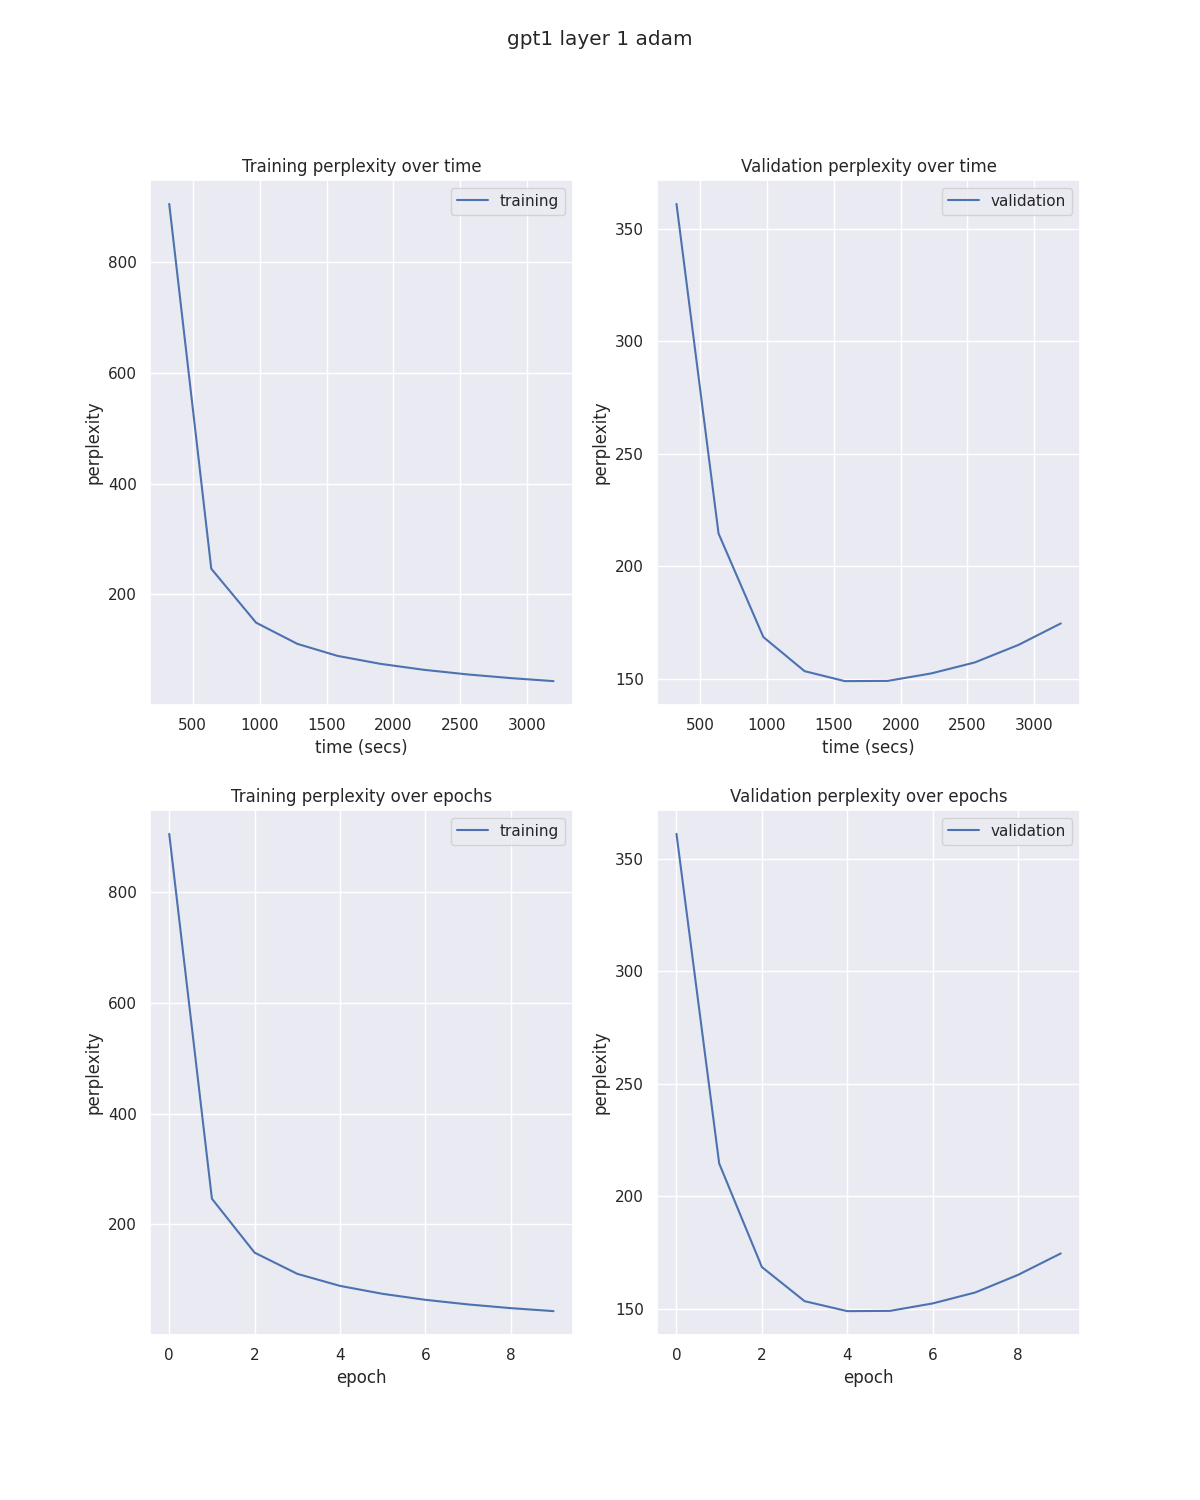
\includegraphics[scale=0.4]{gpt1_layer_1_adam.png}
     \caption{gpt1 with 1 layer and optmized with adam perplexity over time and epochs}
\end{figure}
\begin{figure}[H]
     \centering
     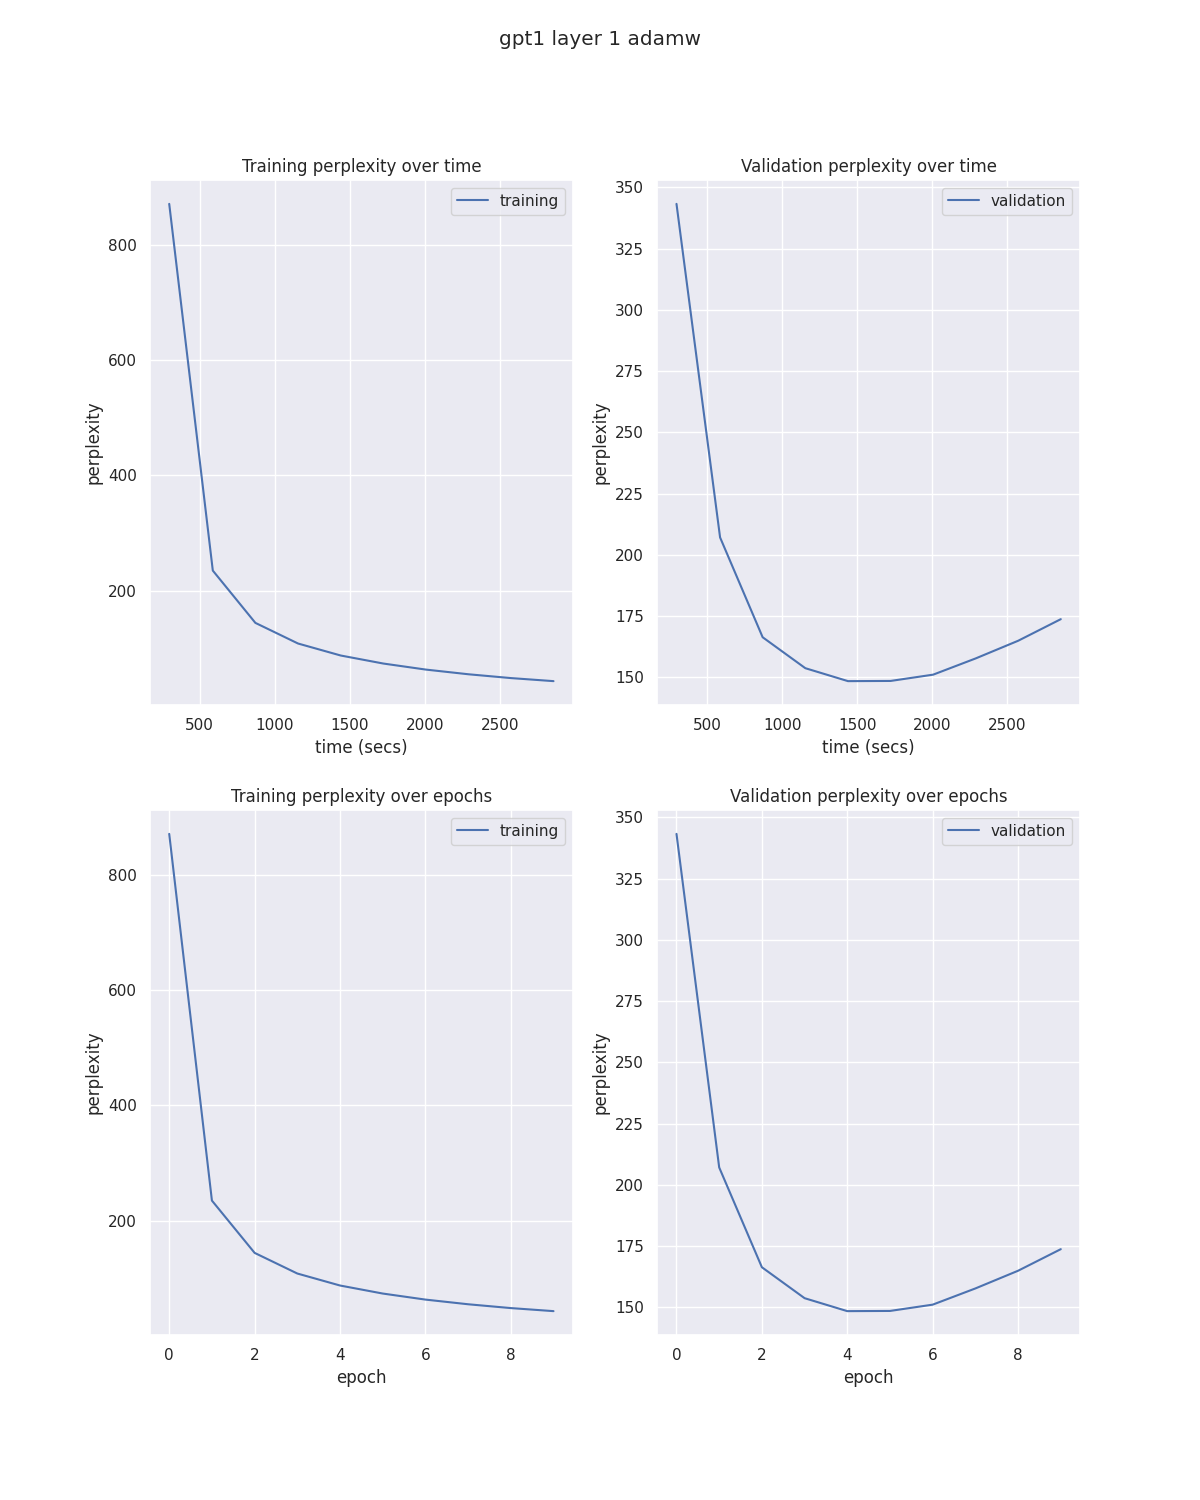
\includegraphics[scale=0.4]{gpt1_layer_1_adamw.png}
     \caption{gpt1 with 1 layer and optmized with adamw perplexity over time and epochs}
\end{figure}
\begin{figure}[H]
     \centering
     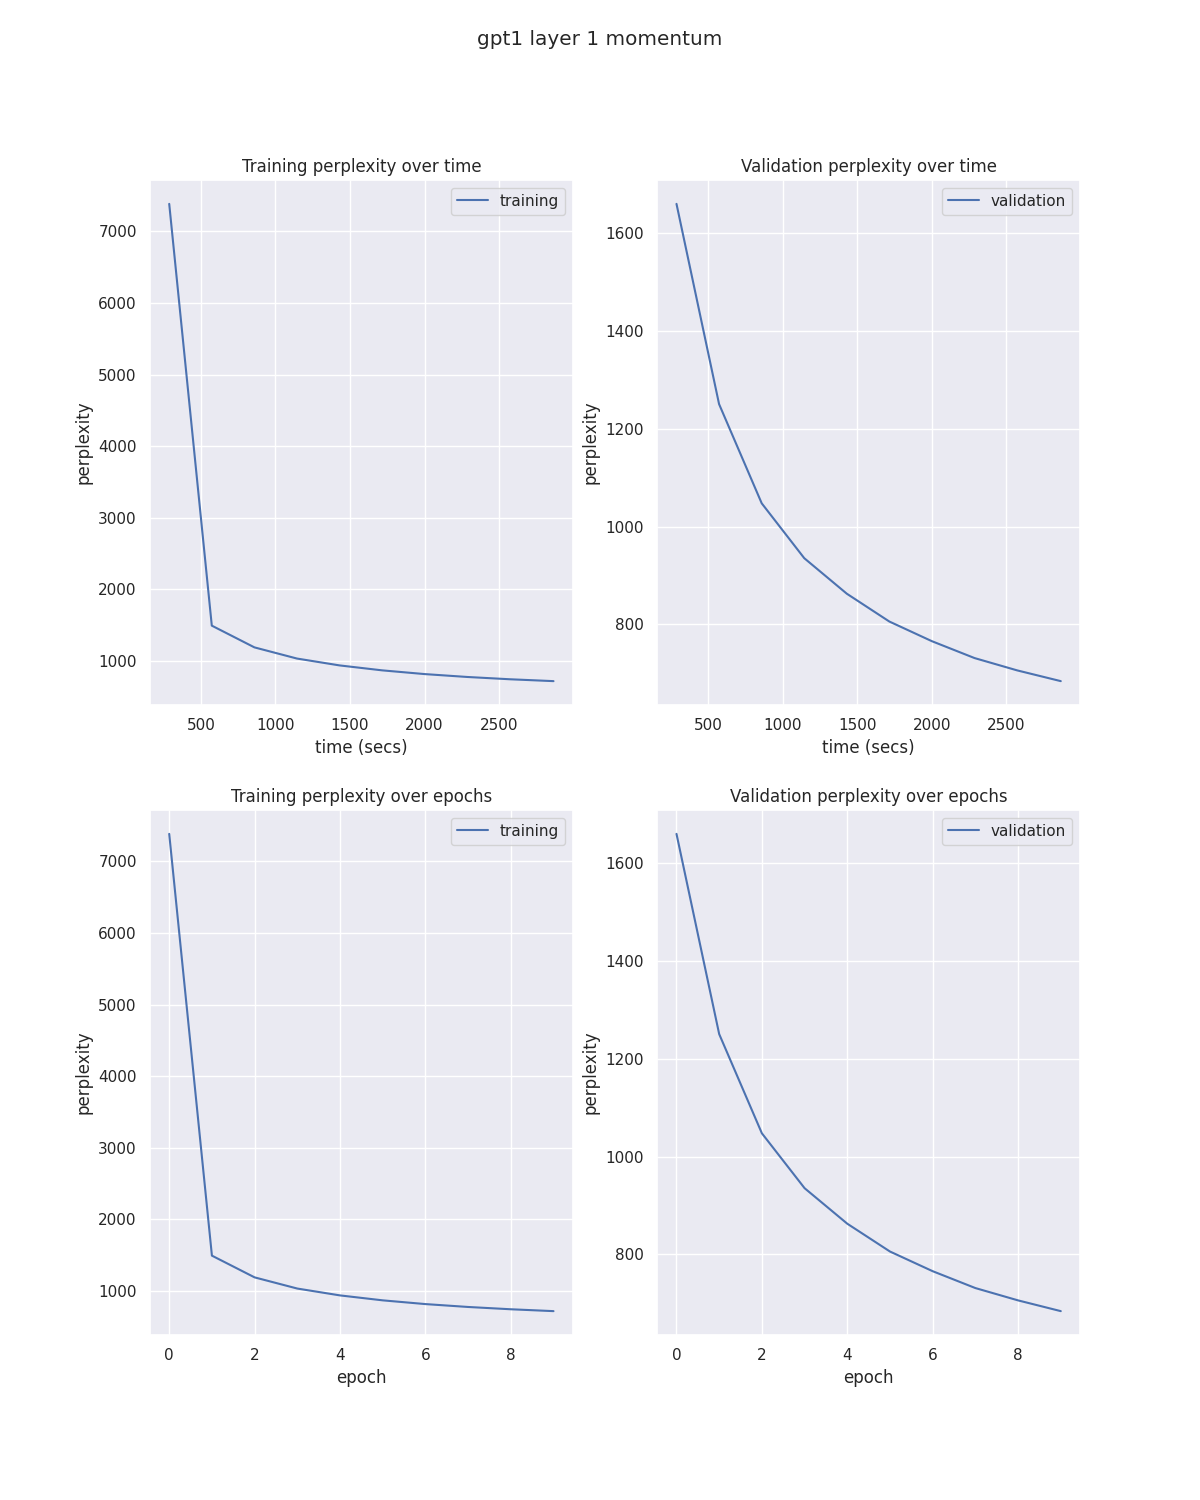
\includegraphics[scale=0.4]{gpt1_layer_1_momentum.png}
     \caption{gpt1 with 1 layer and optmized with momentum perplexity over time and epochs}
\end{figure}
\begin{figure}[H]
     \centering
     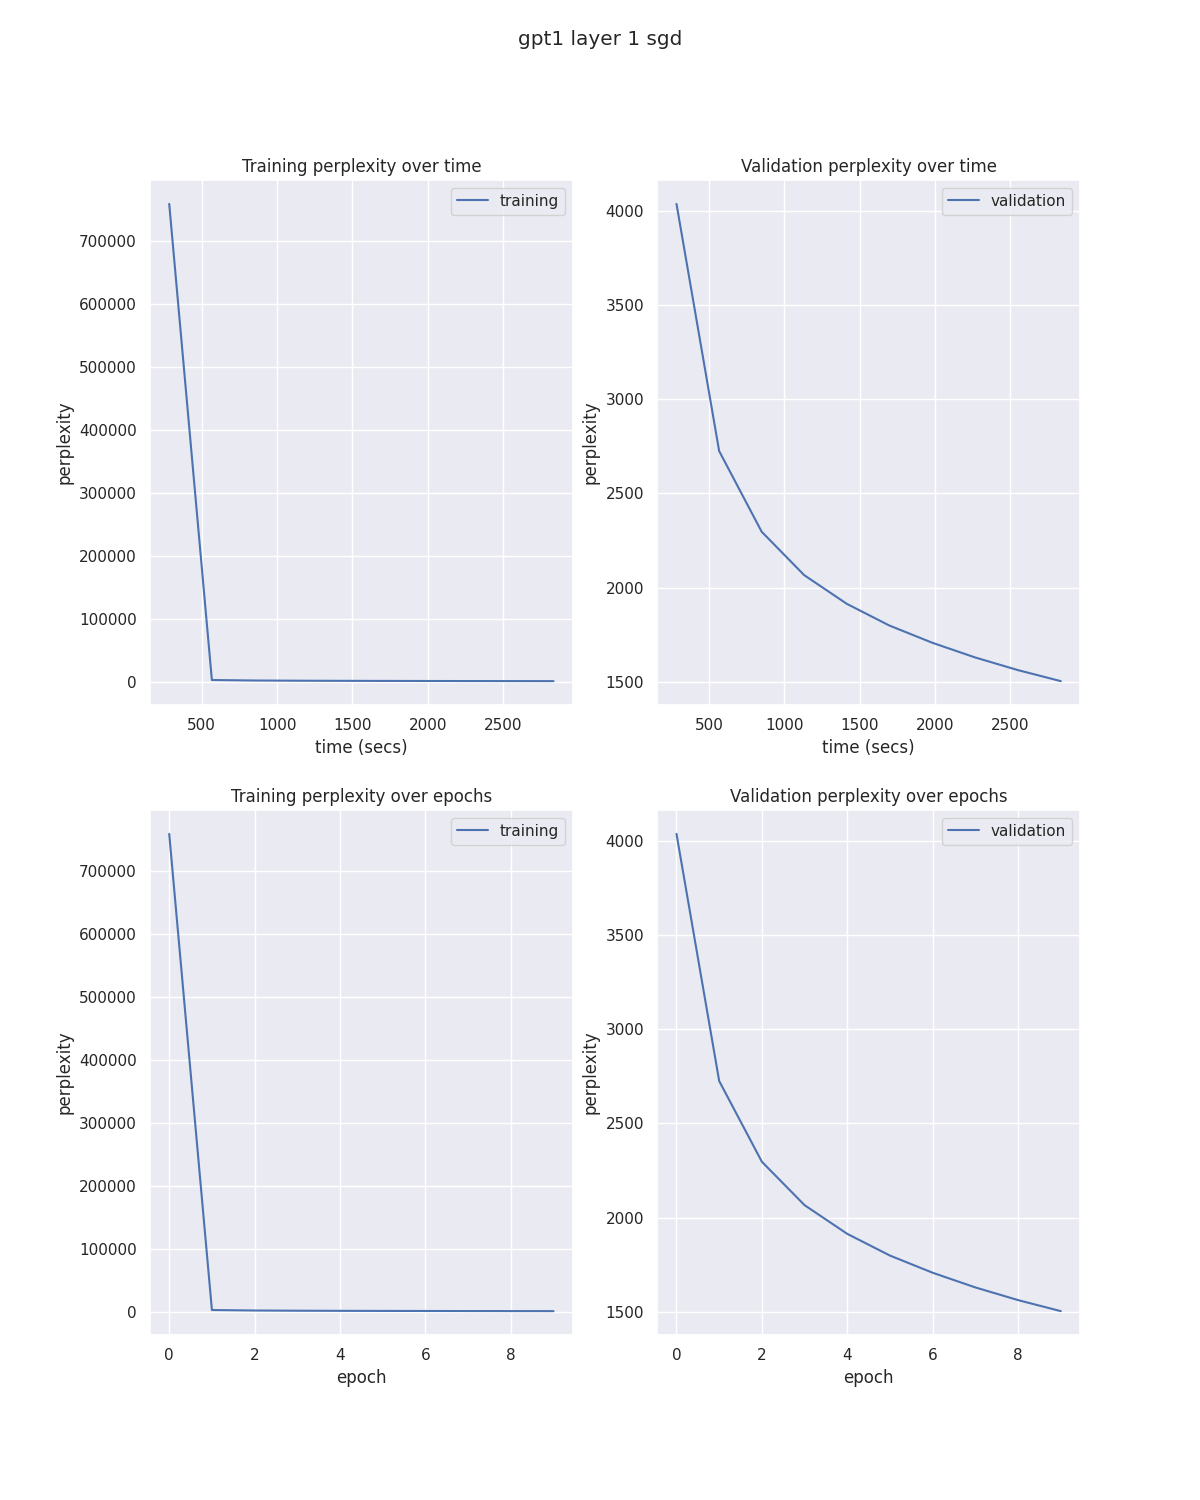
\includegraphics[scale=0.4]{gpt1_layer_1_sgd.png}
     \caption{gpt1 with 1 layer and optmized with sgd perplexity over time and epochs}
\end{figure}
\begin{figure}[H]
     \centering
     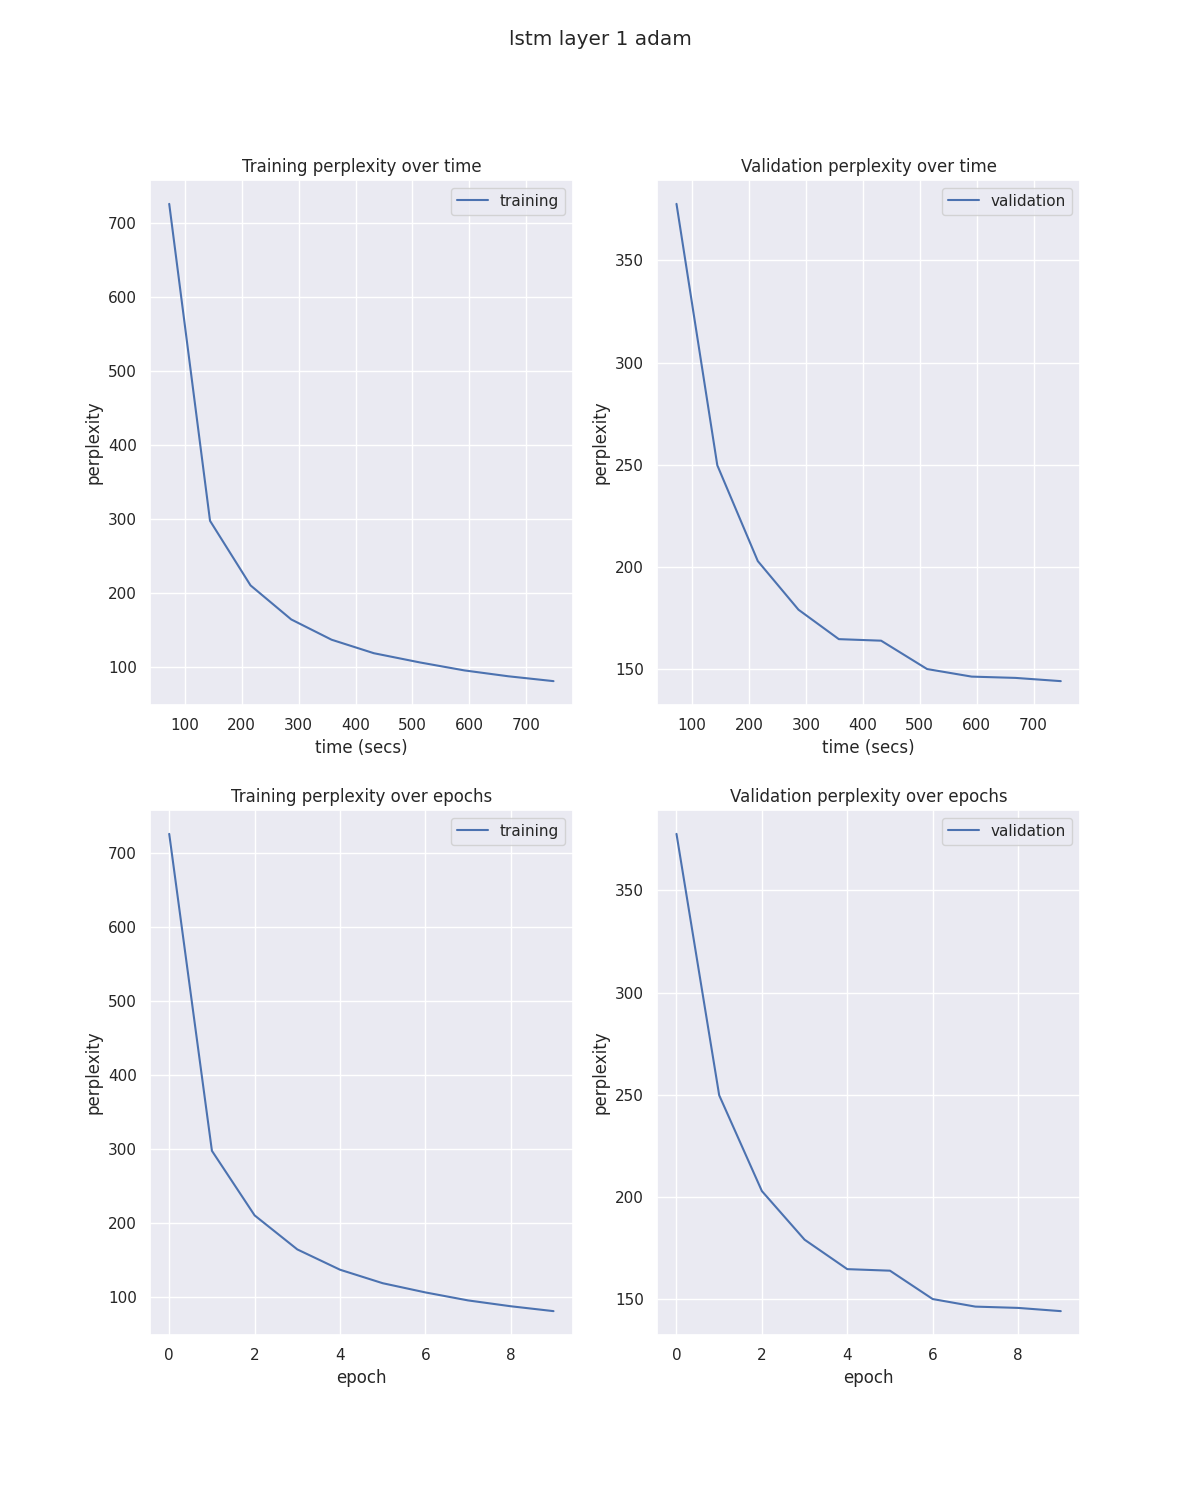
\includegraphics[scale=0.4]{lstm_layer_1_adam.png}
     \caption{lstm with 1 layer and optmized with adam perplexity over time and epochs}
\end{figure}
\begin{figure}[H]
     \centering
     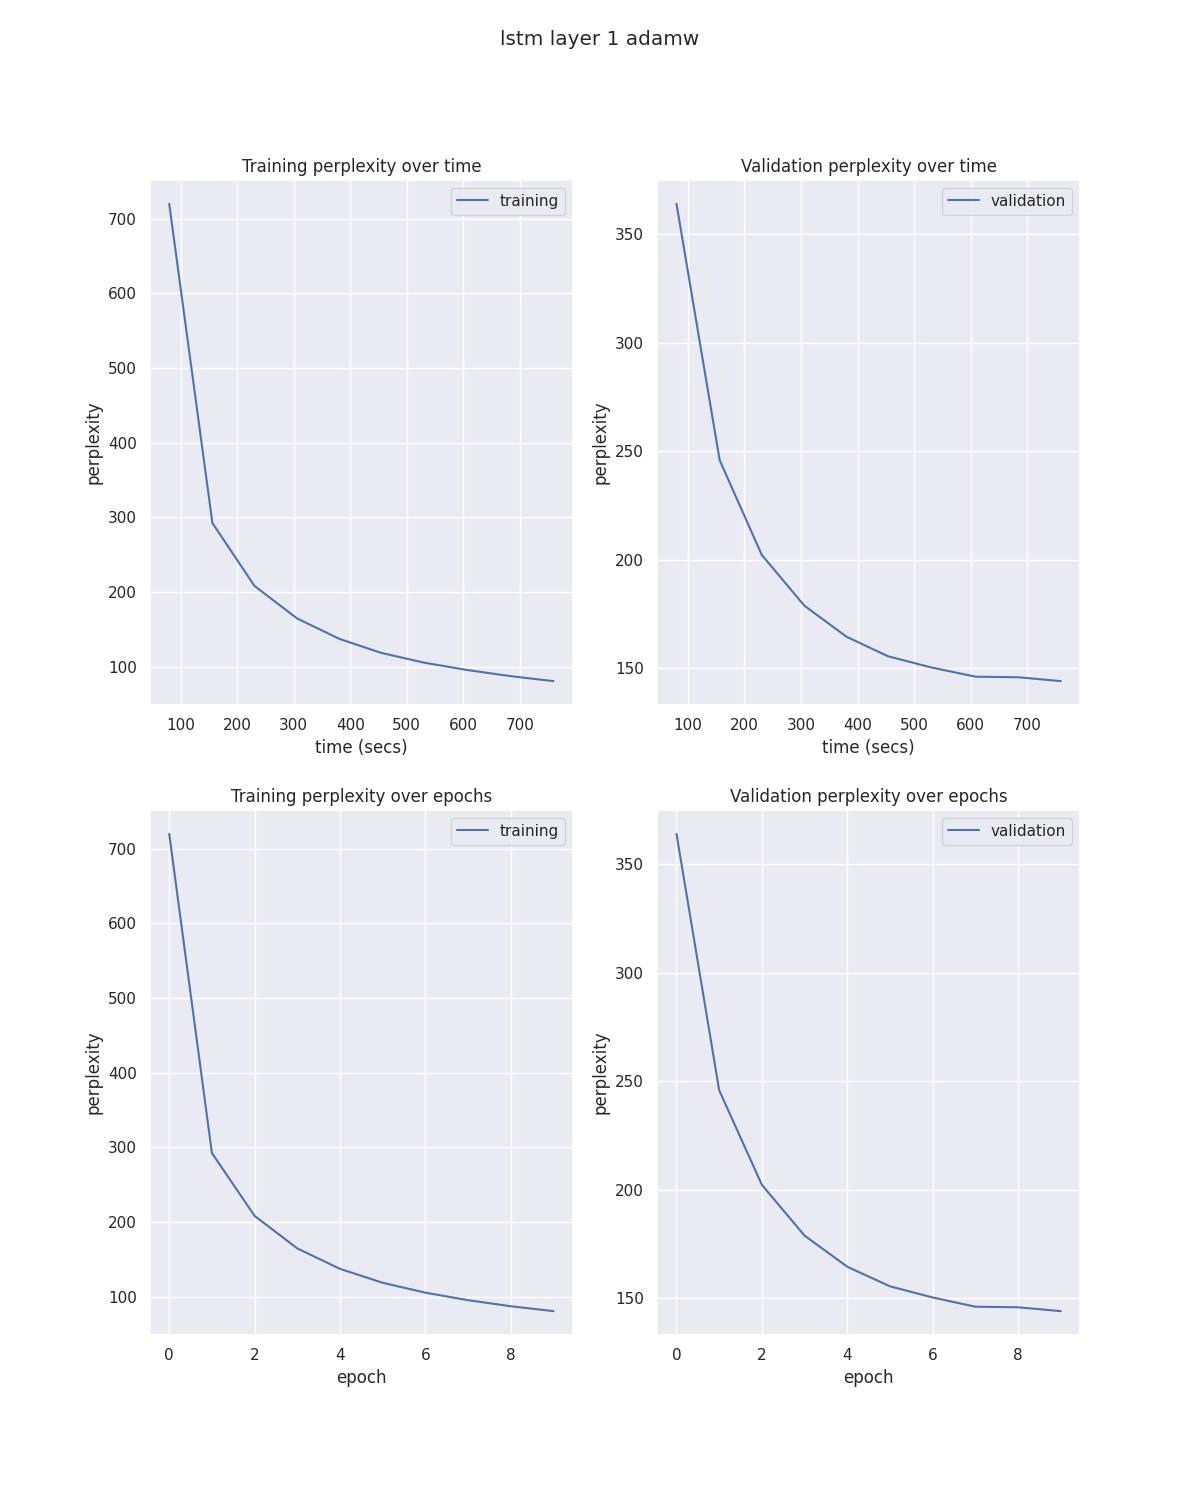
\includegraphics[scale=0.4]{lstm_layer_1_adamw.png}
     \caption{lstm with 1 layer and optmized with adamw perplexity over time and epochs}
\end{figure}
\begin{figure}[H]
     \centering
     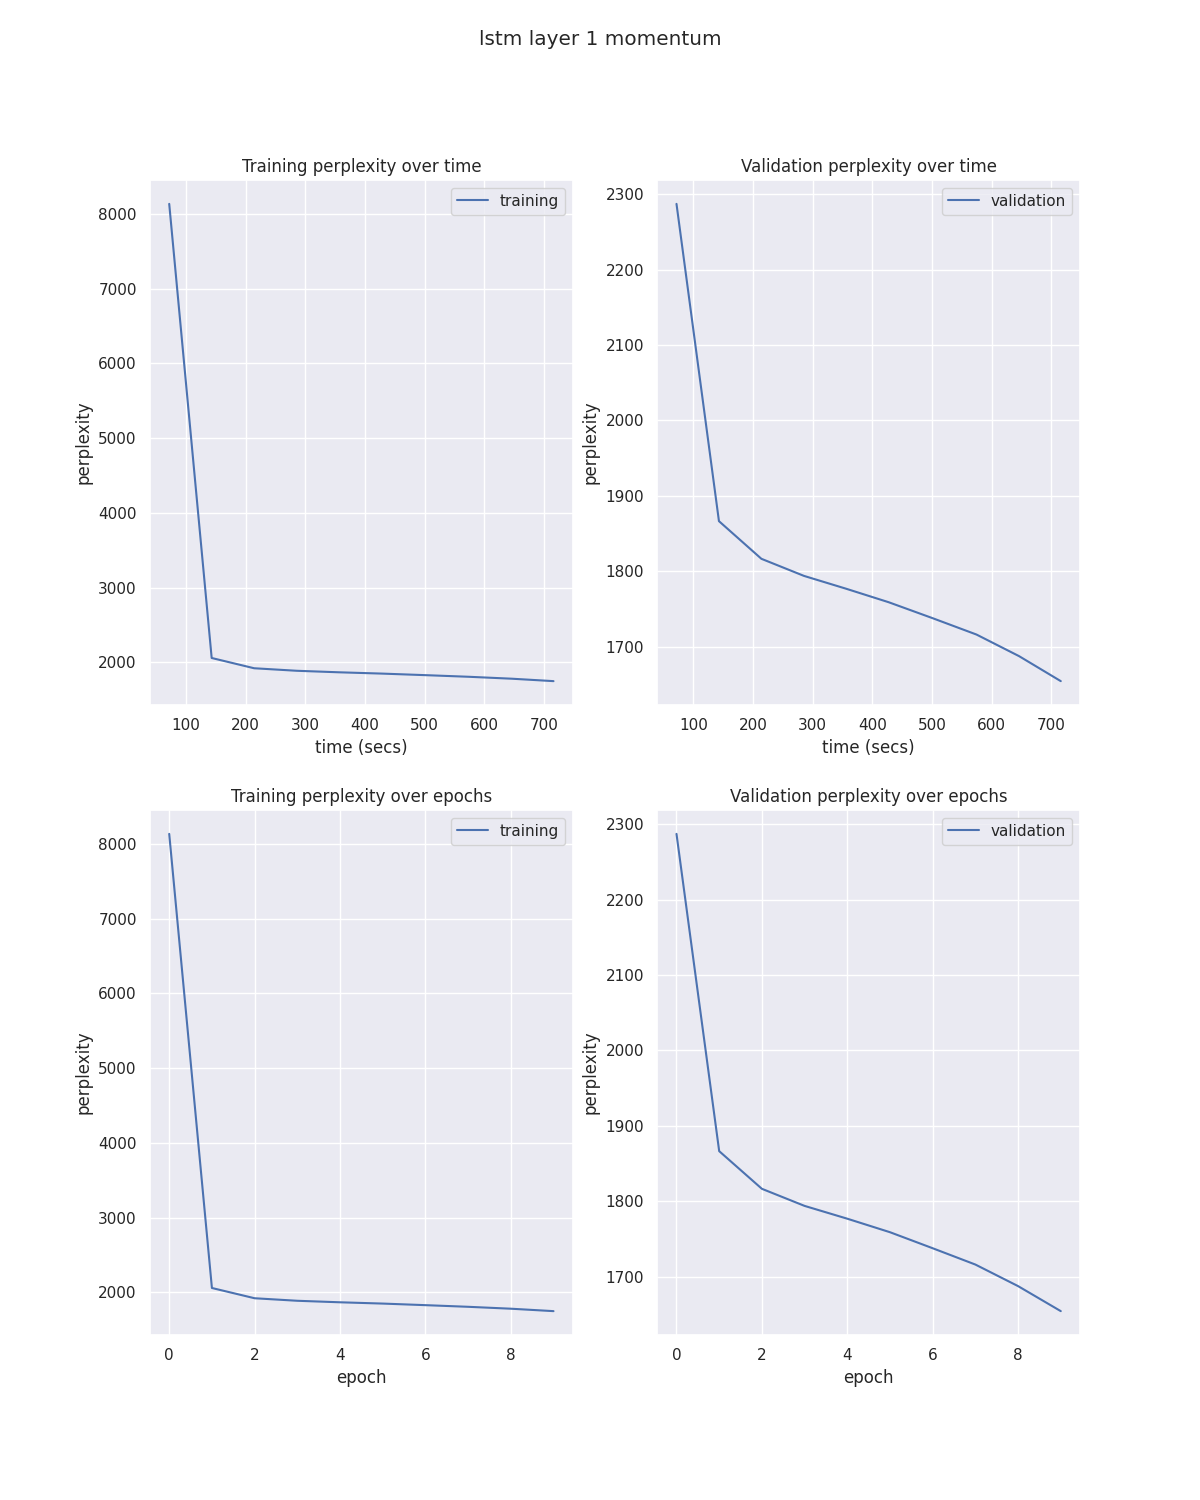
\includegraphics[scale=0.4]{lstm_layer_1_momentum.png}
     \caption{lstm with 1 layer and optmized with momentum perplexity over time and epochs}
\end{figure}
\begin{figure}[H]
     \centering
     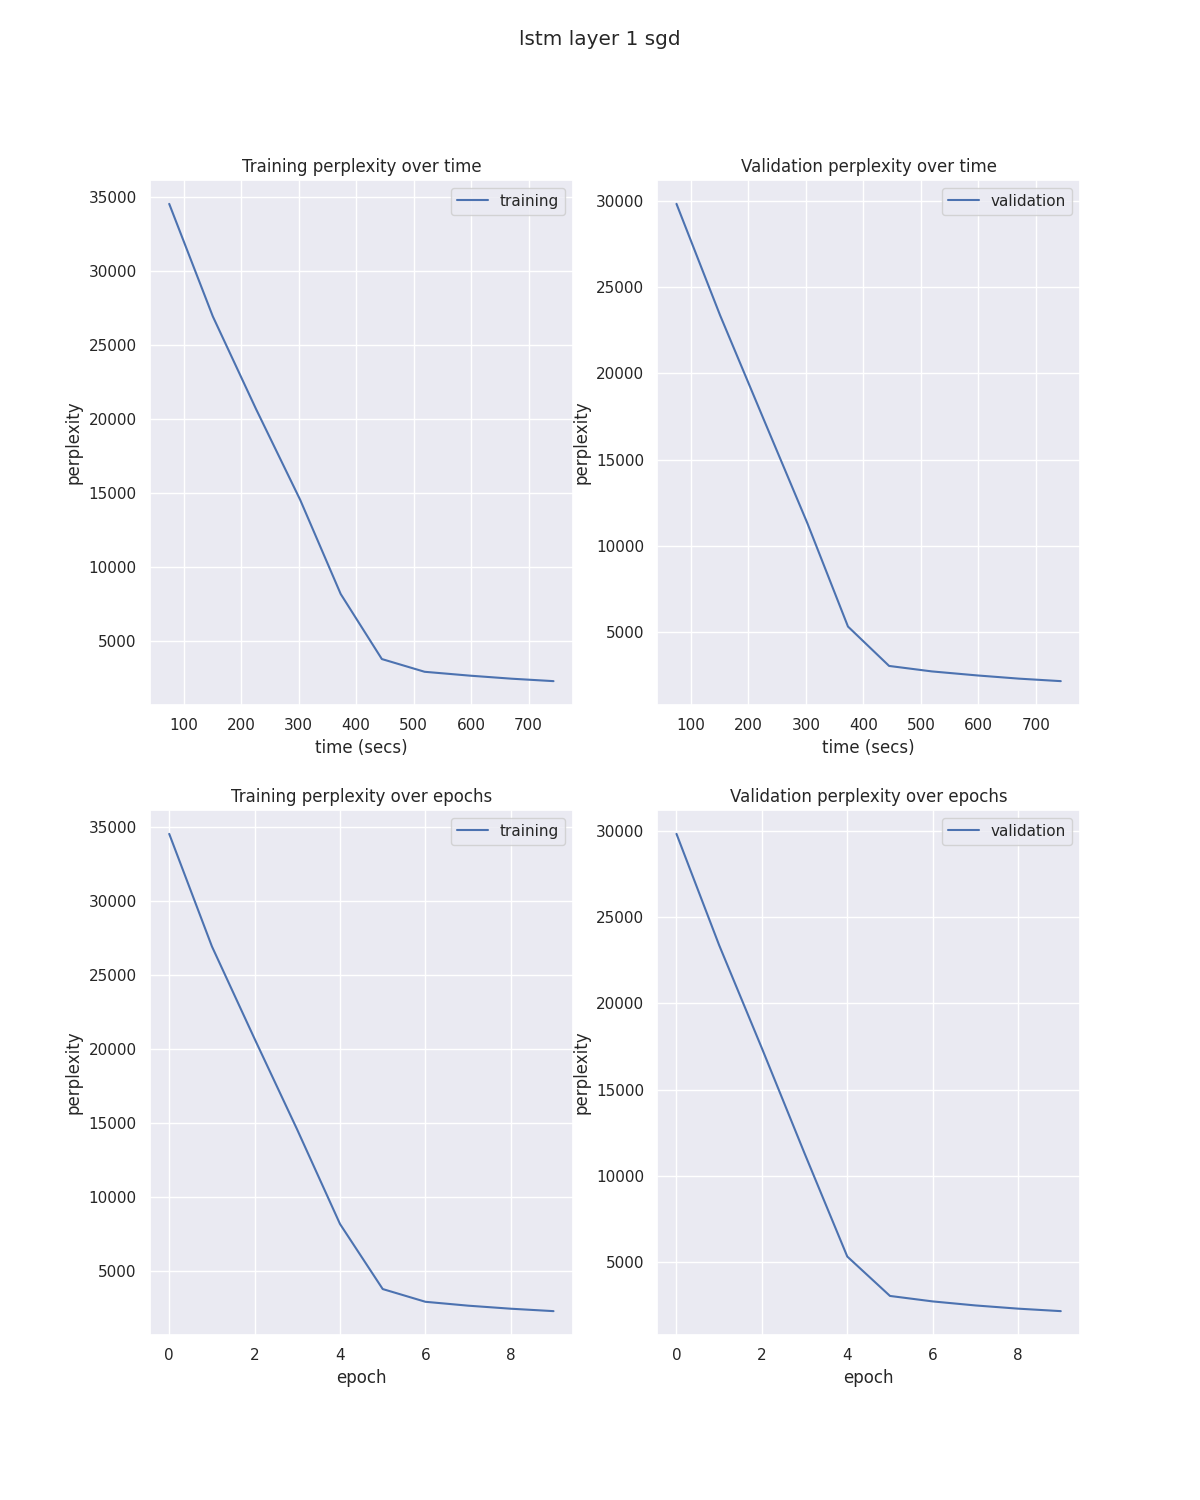
\includegraphics[scale=0.4]{lstm_layer_1_sgd.png}
     \caption{lstm with 1 layer and optmized with sgd perplexity over time and epochs}
\end{figure}
\begin{figure}[H]
     \centering
     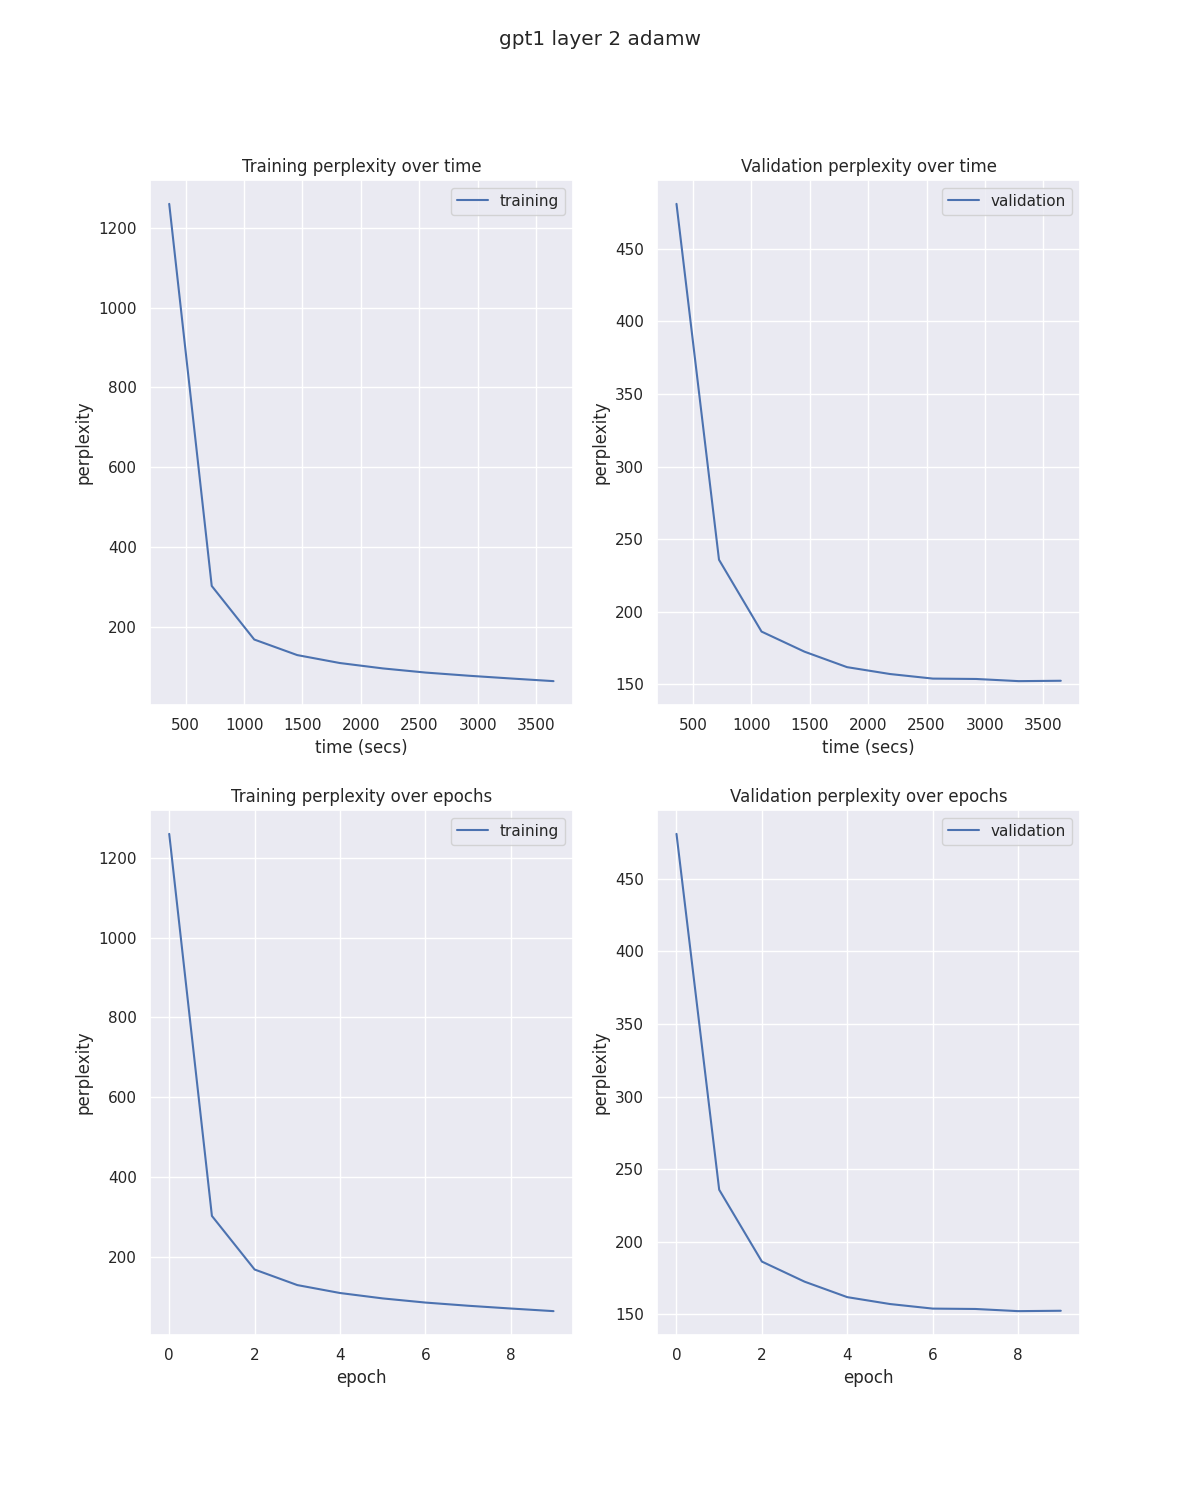
\includegraphics[scale=0.4]{gpt1_layer_2_adamw.png}
     \caption{gpt1 with 2 layer and optmized with adamw perplexity over time and epochs}
\end{figure}
\begin{figure}[H]
     \centering
     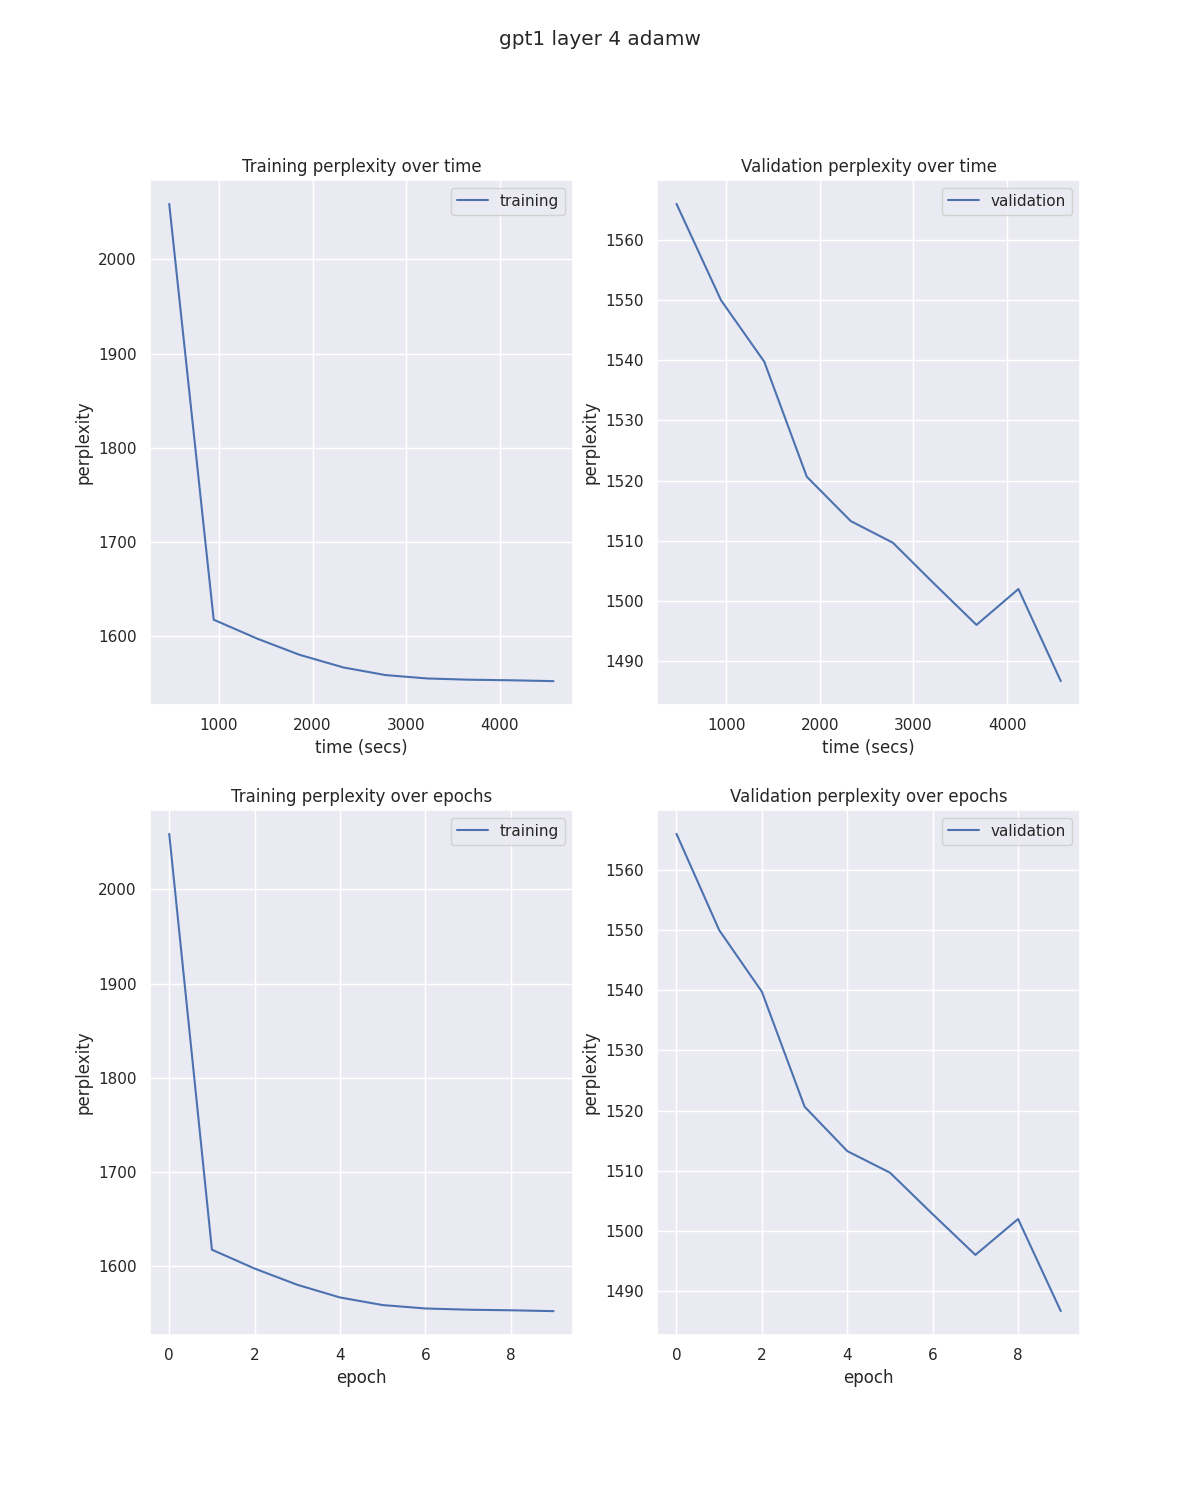
\includegraphics[scale=0.4]{gpt1_layer_4_adamw.png}
     \caption{gpt1 with 4 layer and optmized with adamw perplexity over time and epochs}
\end{figure}
\begin{figure}[H]
     \centering
     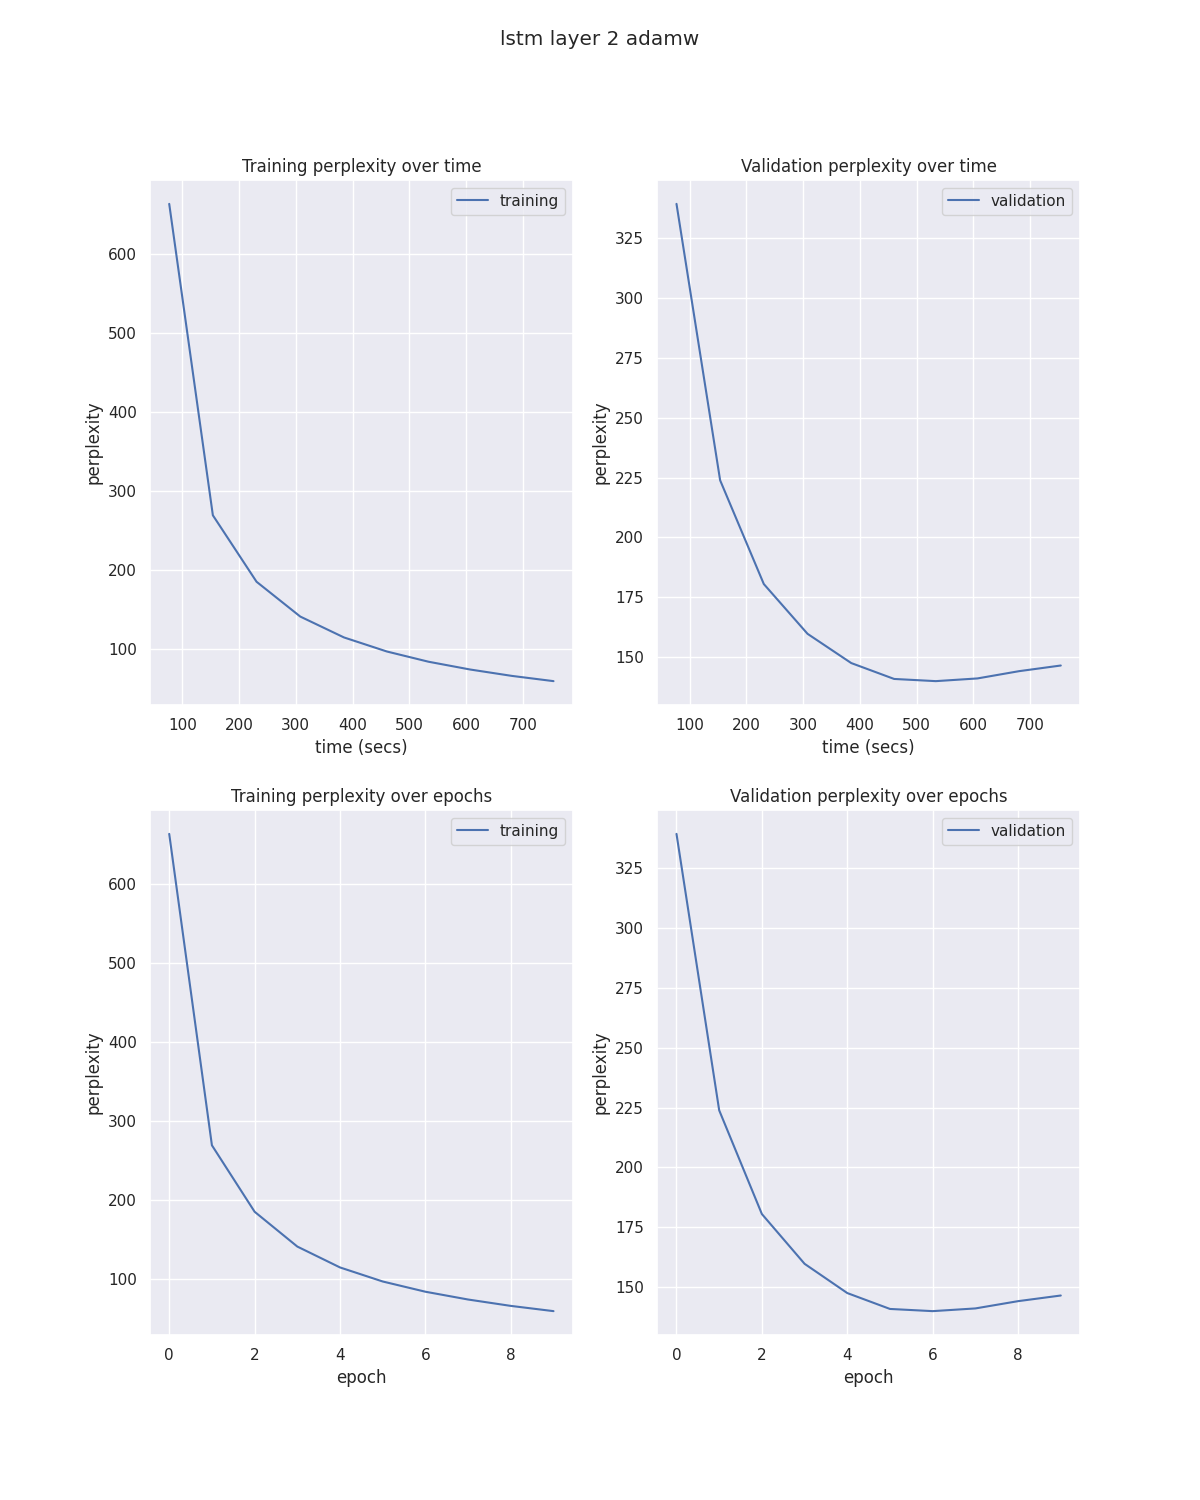
\includegraphics[scale=0.4]{lstm_layer_2_adamw.png}
     \caption{lstm with 2 layer and optmized with adamw perplexity over time and epochs}
\end{figure}
\begin{figure}[H]
     \centering
     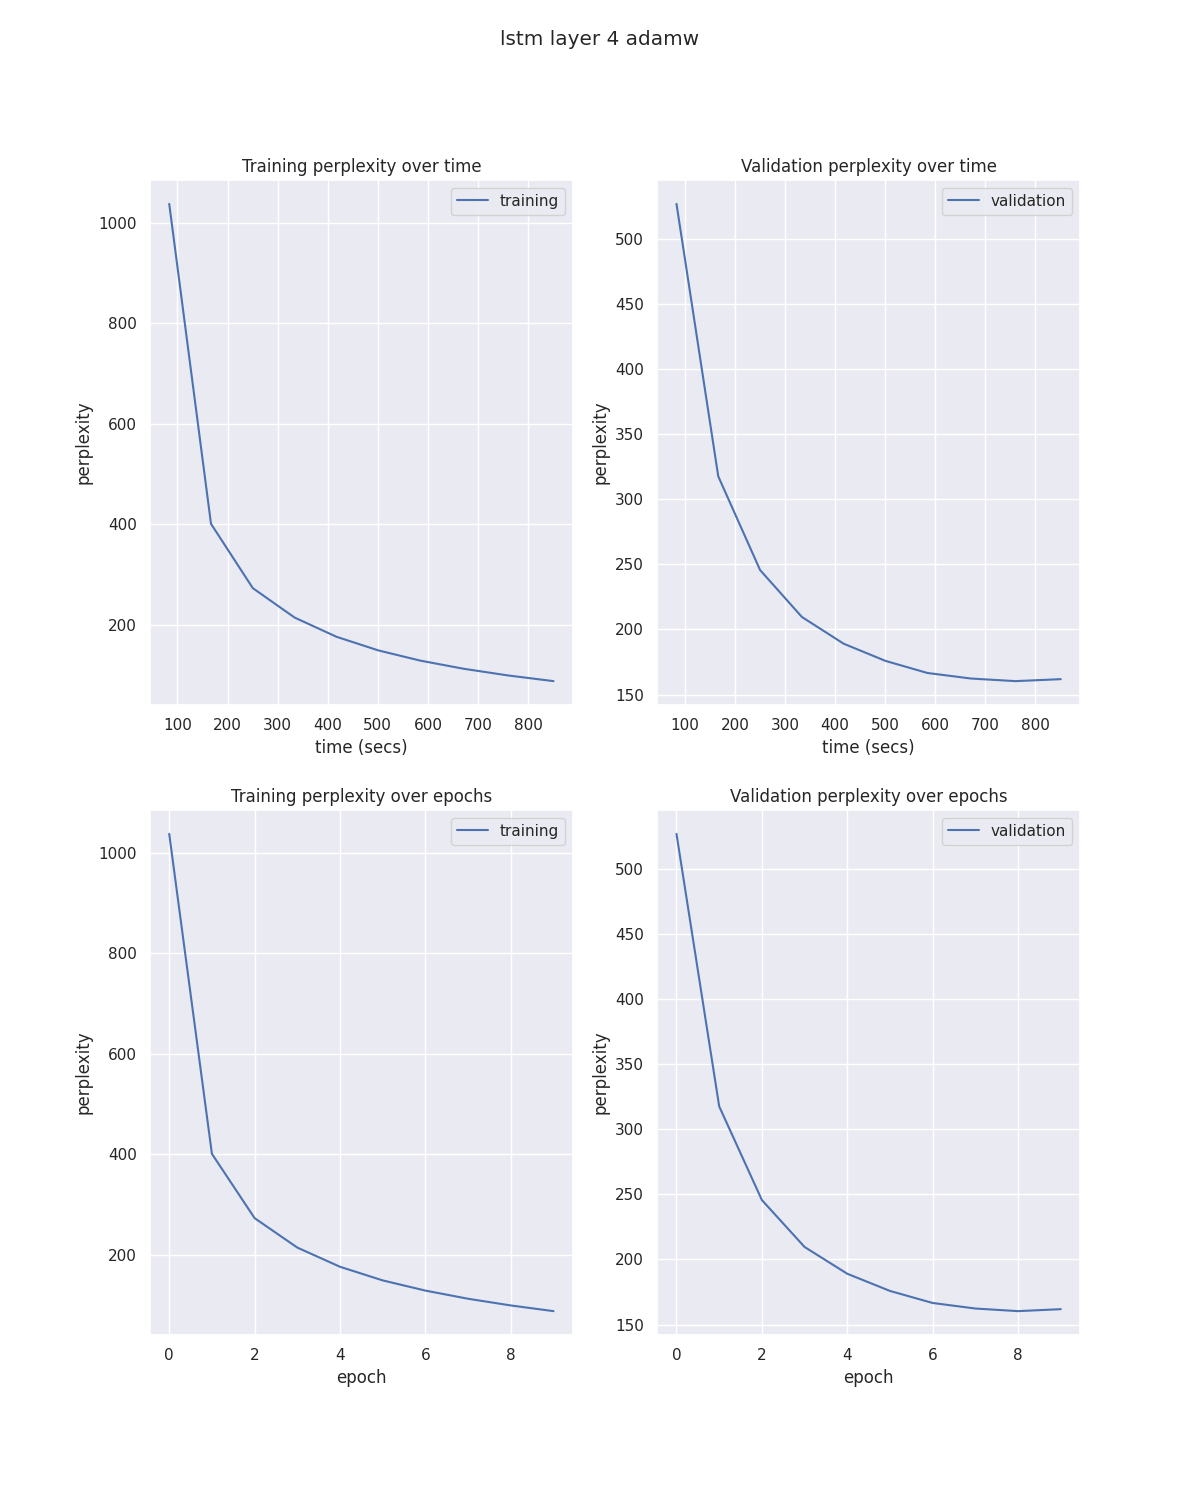
\includegraphics[scale=0.4]{lstm_layer_4_adamw.png}
     \caption{lstm with 4 layer and optmized with adamw perplexity over time and epochs}
\end{figure}

\subsubsection*{Problem 3.2}
Here are the results of the 12 experiments:
\begin{table}[H]
\resizebox{\textwidth}{!}{%
\begin{tabular}{llllllllll}
Exp & Architecture &  \#layers & Optimizer &Train Loss & Train PPL & Validation Loss & Validation PPL & Test Loss & Test PPL \\ \hline
1  & LSTM & 1 & Adam      &4.399 & 81.436 & 4.971 & 144.289 & 4.995 & 147.777 \\
2  & \bf{LSTM} & \bf{1} & \bf{Adamw}     &\bf{4.392} & \bf{80.854} & \bf{4.970} & \bf{144.154} & \bf{5.001} & \bf{148.673} \\
3  & LSTM & 1 & SGD       &7.750 & 2322.216 & 7.684 & 2173.387 &  7.644 & 2088.849 \\
4  & LSTM & 1 & Momentum  &7.446 & 1748.463 & 7.411 & 1654.189 & 7.377 & 1600.139 \\
9  & LSTM & 2 & Adamw     &4.0733 & 58.754 & 4.986 & 146.357 & 5.021 & 151.656 \\
10 & LSTM & 4 & Adamw     &4.470 & 87.406 & 5.086 & 161.846 & 5.106 & 165.131 \\
5  & GPT1 & 1 & Adam      &3.765 & 43.19 & 5.16 & 174.650 & 5.182 & 178.151 \\
6  &\bf{GPT1} & \bf{1}& \bf{Adamw}     &\bf{3.752}&\bf{42.634} &\bf{5.157} & \bf{173.79} & \bf{5.180} & \bf{177.837} \\
7  & GPT1 & 1 & SGD       &7.381 & 1605.992 & 7.315 & 1502.892 & 7.291 & 1467.53 \\
8  & GPT1 & 1 & Momentum  &6.583 & 715.571 & 6.528 & 684.063 & 6.504 & 667.813 \\
11 & GPT1 & 2 & Adamw     &4.167 & 64.525 & 5.026 & 152.330 & 5.023 & 151.896 \\
12 & GPT1 & 4 & Adamw     &7.347 & 1552.593 & 7.304 & 1486.629 & 7.274 & 1443.59
\end{tabular}}
\caption{Results for the 12 experiments. Each models were trained on 10 epochs}
\end{table}

\subsubsection*{Problem 3.3}
If the goal was to minimize the training time of a model, I would choose either
the SGD optimizer or the momentum optmizer with an LSTM. They were the fastest
to train. If the goal was to generalize well, I would chose the LSTM with Adam
or Adamw or GPT1 with Adamw or Adam. These four models had the best test loss for a
single layer model and were all close to each others with respect to the
test loss. Their test perplexity was generally the lowest too.
\subsubsection*{Problem 3.4}
Both SGD and momentum generate high validation perplexity and do not generalize
as well as Adam and Adamw, when comparing the test loss and the test perplexity.
The high precision of Adam and Adamw came at a slightly higher training time.
\subsubsection*{Problem 3.5}
The LSTM performed better for this experiment. It was not yet overfitting, while
the GPT1 model was.  It also had better validation and test perplexity.
\subsubsection*{Problem 3.6}
The result of the transformer architecture are underwhelming. It generally
performed worst than the LSTM architecture. A possible reason is that the LSTM
layers perform better than the transformer layers when there are only a few
number of layers, while the transformers layers scale better when the depth of
the network increases.
\subsubsection*{Problem 3.7}

\end{document}
